\section{The tube transfer}\label{sec:tube}

We first separate the passage to uniformly negative curvature from the
construction of the base metric.  Write $z=(z^1,\ldots,z^{n+1})$ for the
base coordinates and $w=u+iv$ for one additional complex coordinate.
For a smooth real function $\phi$, our metric convention is
\begin{equation}\label{tube:metric-convention}
 |X|_{g_\phi}^{2}
 =\sum_{a,b}\phi_{a\bar b}\,dz^a(X)\overline{dz^b(X)},
 \qquad
 \phi_{a\bar b}=\frac{\partial^2\phi}{\partial z^a\partial\bar z^b}.
\end{equation}
Thus the potential $|z|^2$ gives the Euclidean real metric, without an
additional factor of two.  We use
\[
 d^c\phi=-d\phi\circ J=i(\bar\partial\phi-\partial\phi),
 \qquad 2\partial\phi=d\phi+i\,d^c\phi.
\]
The real curvature tensor is normalized so that
$R(X,Y,Y,X)$ is the sectional-curvature numerator and the unit sphere
has positive curvature.

\begin{lemma}[Tube transfer]\label{tube:transfer}
Let $\ell\colon\mathbb C^{n+1}\to\mathbb R$ be smooth and strictly
plurisubharmonic.  Suppose that its potential metric $g_\ell$, in
Convention~\eqref{tube:metric-convention}, is complete and has
nonpositive real sectional curvature.  Set
\begin{equation}\label{tube:domain}
 \mathcal T_\ell
 =\{(z,w)\in\mathbb C^{n+1}\times\mathbb C:
           b(z,w):=\operatorname{Im}w-\ell(z)>0\},
 \qquad g_{\mathcal T}=g_{-\log b}.
\end{equation}
Then $\mathcal T_\ell$ is connected and simply connected, indeed
diffeomorphic to $\mathbb R^{2n+4}$, and $g_{\mathcal T}$ is a complete
K\"ahler metric satisfying
\[
 \operatorname{Sec}_{g_{\mathcal T}}\le -1.
\]
No lower curvature bound on $g_\ell$ is required.
\end{lemma}

\begin{proof}
\emph{Topology and the metric.}
The map
\[
 (z,u,b)\longmapsto (z,u+i(\ell(z)+b))
\]
is a smooth diffeomorphism from
$\mathbb C^{n+1}\times\mathbb R\times(0,\infty)$ onto $\mathcal T_\ell$.
The claimed topology follows, for example by using $\log b$ as the last
real coordinate.

Let $\pi(z,w)=z$.  Differentiating the potential gives, as Hermitian
forms,
\begin{equation}\label{tube:complex-decomposition}
 g_{\mathcal T}
 =b^{-1}\pi^*g_\ell+b^{-2}\partial b\otimes\bar\partial b.
\end{equation}
Here $d^cv=-du$, and consequently
\[
 2\partial b=db-i(du+d^c\ell).
\]
In real notation Equation~\eqref{tube:complex-decomposition} is
\begin{equation}\label{tube:real-decomposition}
 \boxed{\quad
 g_{\mathcal T}
 =b^{-1}\pi^*g_\ell
   +\frac{db^2+(du+d^c\ell)^2}{4b^2}.
 \quad}
\end{equation}
The pullback in the first term is implicit when evaluating forms from
the base.  In particular, the sign before $d^c\ell$ is positive with
the convention above.  Formula~\eqref{tube:complex-decomposition} is
positive definite: its first summand controls the base component, and
on a vector with zero base component its second summand controls the
remaining complex $w$ component.  Being the complex Hessian of a
smooth potential, it is K\"ahler.

\begin{figure}[tb]
 \centering
 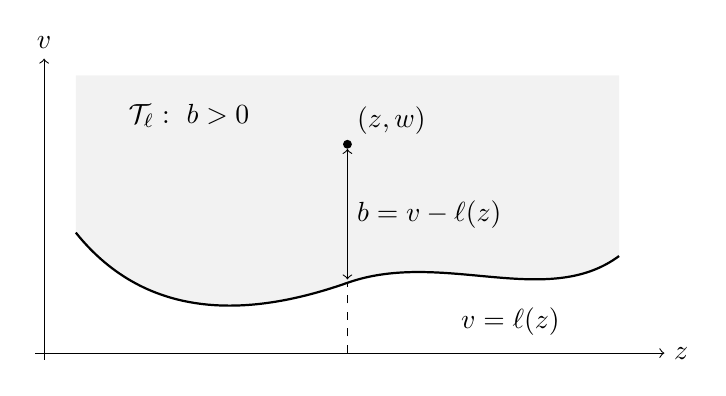
\begin{tikzpicture}[x=1.15cm,y=.85cm]
 \fill[black!5]
  (-3,1.8) .. controls (-2.2,.45) and (-1.05,.55) .. (0,1.05)
  .. controls (1.05,1.55) and (2.2,.65) .. (3,1.45)
  -- (3,4.15) -- (-3,4.15) -- cycle;
 \draw[->] (-3.45,0) -- (3.5,0) node[right] {$z$};
 \draw[->] (-3.35,-.1) -- (-3.35,4.4) node[above] {$v$};
 \draw[thick]
  (-3,1.8) .. controls (-2.2,.45) and (-1.05,.55) .. (0,1.05)
  .. controls (1.05,1.55) and (2.2,.65) .. (3,1.45);
 \node[anchor=north] at (1.8,.82) {$v=\ell(z)$};
 \draw[dashed] (0,0) -- (0,1.05);
 \draw[<->] (0,1.1) -- (0,3.05)
  node[midway,right] {$b=v-\ell(z)$};
 \fill (0,3.12) circle (1.6pt);
 \node[above right] at (0,3.12) {$(z,w)$};
 \node at (-1.75,3.55) {$\mathcal T_\ell:\ b>0$};
\end{tikzpicture}

 \caption{A schematic real slice of the tube.  The coordinate
 $b=v-\ell(z)$ is the positive vertical gap; $u$ and the other base
 directions are suppressed.  No convexity of the graph is assumed.}
 \label{tube:geometry}
\end{figure}

\emph{Completeness.}
Let $\gamma$ be a locally piecewise smooth curve of finite
$g_{\mathcal T}$-length, with its parameter tending to an endpoint.
Equation~\eqref{tube:real-decomposition} gives
\[
 \frac{|db(\dot\gamma)|}{2b}\le |\dot\gamma|_{g_{\mathcal T}}.
\]
Thus $\log b$ has finite total variation.  In particular, along this
curve there are constants $0<b_-\le b\le b_+<\infty$, and $b$ has a
positive limit.  The same metric identity implies
\[
 |(\pi\circ\gamma)'|_{g_\ell}
 \le \sqrt{b_+}\,|\dot\gamma|_{g_{\mathcal T}}.
\]
The base projection therefore has finite length and converges by
completeness of $g_\ell$.  Its image has compact closure.  On that
compact set $|d^c\ell|_{g_\ell}$ is bounded by some constant $C$, so
\[
 |u'|
 \le |(du+d^c\ell)(\dot\gamma)|
       +|d^c\ell((\pi\circ\gamma)')|
 \le 2b_+|\dot\gamma|_{g_{\mathcal T}}
       +C|(\pi\circ\gamma)'|_{g_\ell}.
\]
Hence $u$ also converges.  Since $v=b+\ell(z)$, the curve has a limit
in $\mathcal T_\ell$.  This finite-length criterion proves metric
completeness.  Indeed, a Cauchy sequence without a limit would have a
subsequence whose successive distances are less than $2^{-j}$;
joining successive points by paths of length less than $2^{1-j}$
would produce a finite-length curve without a limit.

\emph{The curvature comparison.}
For a Hermitian matrix $g=(g_{a\bar b})$ arising from a K\"ahler
potential, denote its Hermitian curvature components by
\begin{equation}\label{tube:hermitian-curvature}
 \mathcal R^g_{a\bar b c\bar d}
 =-\partial_a\partial_{\bar b}g_{c\bar d}
   +\sum_{p,q}g^{p\bar q}
       (\partial_a g_{c\bar q})(\partial_{\bar b}g_{p\bar d}).
\end{equation}
We record explicitly how these components determine the real
sectional numerator in our normalization.  If
$\xi^a=dz^a(X)$ and $\eta^a=dz^a(Y)$, set
\[
 T^{a\bar b}=i(\xi^a\bar\eta^b-\eta^a\bar\xi^b).
\]
Expansion of $X=\sum_a(\xi^a\partial_{z^a}
+\bar\xi^a\partial_{\bar z^a})$ and similarly of $Y$, using the
K\"ahler curvature symmetries, gives
\begin{align}
 R_g(X,Y,Y,X)
 &=\mathcal R^g(\xi,\bar\xi,\eta,\bar\eta)
   -\operatorname{Re}\mathcal R^g(\xi,\bar\eta,\xi,\bar\eta)
       \label{tube:real-complex-curvature}\\
 &=\frac12\sum_{a,b,c,d}
        \mathcal R^g_{a\bar b c\bar d}
        T^{a\bar b}T^{c\bar d}.\nonumber
\end{align}
The factor $1/2$ reflects that the complexification of the real
metric satisfies
$g(\partial_{z^a},\partial_{\bar z^b})=g_{a\bar b}/2$.

Fix a point of the tube over a base point $z_0$.  Choose holomorphic
K\"ahler normal coordinates on the base, centered at $z_0$, so that
$(\ell_{a\bar b})$ is the identity and its first derivatives vanish
there.  Such coordinates follow by a linear normalization followed
by a quadratic holomorphic change of coordinates; the K\"ahler
symmetry makes the quadratic coefficients symmetric in their two
holomorphic indices.  The mixed terms of total degree three in the
potential then vanish.  Subtracting the real part of a holomorphic
polynomial of degree at most three removes its remaining nonconstant
pure terms.  This subtraction is absorbed by a holomorphic
translation of $w$: if $\ell=\ell_0+\operatorname{Re}H$, replace
$w$ by $w-iH$.  Thus in the adapted coordinates the base potential
has three-jet
\[
 c+|z|^2.
\]

Compare the tube potential at this point with
\begin{equation}\label{tube:model-potential}
 \Phi_0=-\log(\operatorname{Im}w-c-|z|^2).
\end{equation}
The two metrics and their first derivatives agree at the point.
Their cubic contractions in
Equation~\eqref{tube:hermitian-curvature} therefore agree.  In the
fourth potential derivatives the only difference is the term
$b^{-1}\ell_{a\bar b c\bar d}$ with all four indices in the base.
The base cubic contractions vanish in the normal coordinates, so
\begin{equation}\label{tube:hermitian-transfer}
 \mathcal R^{g_{\mathcal T}}-\mathcal R^{g_{\Phi_0}}
 =b^{-1}\pi^*\mathcal R^{g_\ell}
 \qquad\text{at the comparison point}.
\end{equation}
Applying Equation~\eqref{tube:real-complex-curvature} gives the
corresponding identity of real sectional numerators:
\begin{equation}\label{tube:real-transfer}
 \begin{split}
 R_{g_{\mathcal T}}(X,Y,Y,X)
 &=R_{g_{\Phi_0}}(X,Y,Y,X)\\
 &\quad+b^{-1}R_{g_\ell}(d\pi X,d\pi Y,d\pi Y,d\pi X).
 \end{split}
\end{equation}
In particular, the extra term is nonpositive for every real pair
$X,Y$.  This remains true when their base projections are linearly
dependent, in which case that term is zero.  The comparison metrics
agree at the point, so the sectional-curvature denominators also
agree.

\emph{The model normalization.}
Put $\widetilde w=w-ic$.  The Cayley coordinates
\[
 (\mathcal Z,\mathcal W)
 =\left(\frac{2z}{\widetilde w+i},
         \frac{\widetilde w-i}{\widetilde w+i}\right)
\]
satisfy
\[
 1-|\mathcal Z|^2-|\mathcal W|^2
 =\frac{4(\operatorname{Im}\widetilde w-|z|^2)}
        {|\widetilde w+i|^2}.
\]
Consequently the potential in Equation~\eqref{tube:model-potential}
equals $-\log(1-|\mathcal Z|^2-|\mathcal W|^2)$ up to a
pluriharmonic summand and a constant.  Our comparison point has
$z=0$.  A real translation of $\widetilde w$ and a dilation
$(z,\widetilde w)\mapsto(z/\sqrt r,\widetilde w/r)$, $r>0$, are
model isometries and place it at $(0,i)$, which the Cayley map sends
to the ball origin.

Writing $Z$ for all the ball coordinates, expansion of
$-\log(1-|Z|^2)$ at zero gives
\[
 g_{a\bar b}(0)=\delta_{ab},\qquad
 \partial g_{a\bar b}(0)=0,\qquad
 \mathcal R^{g_{\Phi_0}}_{a\bar b c\bar d}(0)
 =-(\delta_{ab}\delta_{cd}+\delta_{ad}\delta_{cb}).
\]
For real orthonormal $X,Y$ at the origin, their complex components
$\xi,\eta$ have norm one and satisfy
$\operatorname{Re}\langle\xi,\eta\rangle=0$.  Write
$\langle\xi,\eta\rangle=i\beta$, where $|\beta|\le1$.
Equation~\eqref{tube:real-complex-curvature} now gives
\begin{equation}\label{tube:model-sectional}
 \operatorname{Sec}_{g_{\Phi_0}}(X\wedge Y)
 =-1-3\beta^2\in[-4,-1].
\end{equation}
Combining Equations~\eqref{tube:real-transfer}
and~\eqref{tube:model-sectional} proves
$\operatorname{Sec}_{g_{\mathcal T}}\le-1$ on all real planes.
\end{proof}

The same comparison also explains why this construction need not
have a lower sectional-curvature bound.

\begin{corollary}\label{tube:negative-plane}
Under the hypotheses of Lemma~\ref{tube:transfer}, suppose that
$g_\ell$ has a real two-plane of strictly negative sectional
curvature at some point.  Then
\[
 \inf\operatorname{Sec}_{g_{\mathcal T}}=-\infty.
\]
\end{corollary}

\begin{proof}
Let $X,Y$ be an orthonormal basis of such a base plane $\sigma$.
At a point above it with height $b$, the distribution
\[
 \mathcal H=\ker db\cap\ker(du+d^c\ell)
\]
is $J$-invariant, and $d\pi$ identifies its metric with
$b^{-1}g_\ell$.  If $\widehat X,\widehat Y$ are the horizontal lifts
of $X,Y$, then $\sqrt b\,\widehat X,\sqrt b\,\widehat Y$ are
$g_{\mathcal T}$-orthonormal.  Equation~\eqref{tube:real-transfer}
and the model computation give the exact formula
\[
 \operatorname{Sec}_{g_{\mathcal T}}
   (\widehat X\wedge\widehat Y)
 =-1-3g_\ell(JX,Y)^2+b\operatorname{Sec}_{g_\ell}(\sigma).
\]
Letting $b\to\infty$ proves the assertion.
\end{proof}
